\documentclass[]{beamer}
\usepackage{tikz}
\usepackage{pgfplots}
\usepackage[dutch]{babel}
\usepackage[T1]{fontenc}
\usepackage{graphicx}
\usepackage{braket}
\usepackage{color}
\usepackage{xcolor}
\usepackage{wrapfig}
\usepackage{amsmath}
\renewcommand{\thefootnote}{}
\addtolength{\jot}{1em}
\renewcommand{\familydefault}{\sfdefault}
\renewcommand*\sfdefault{lmss}

\definecolor{green}{rgb}{0.24,0.60,0.34}
\definecolor{purple}{rgb}{0.60,0.24,0.44}

\newsavebox\MBox
\newcommand\Cline[2][red]{{\sbox\MBox{$#2$}%
  \rlap{\usebox\MBox}\color{#1}\rule[-1.2\dp\MBox]{\wd\MBox}{0.5pt}}}

\makeatletter
\def\beamer@origitem{%
  \@inmatherr\item\@ifnextchar[\@item{\@noitemargtrue\@item[\@itemlabel]%
  \csname beamer@thcfg@\beameritemnestingprefix item\endcsname% Insert colour in \beamer@thc@fg
  \ifx\beamer@thc@fg\@empty\relax\else\color{\beamer@thc@fg}\fi% Execute colour
 }}
\makeatother

\begin{document}
\usetikzlibrary{snakes, shapes, calc}
\usetikzlibrary{mindmap,trees, matrix}
\tikzset{every concept/.style={minimum size=2cm, text width=2cm}}
\tikzset{
  ashadow/.style={opacity=.45, shadow xshift=0.07, shadow yshift=-0.07},
}

\setbeamercolor{background canvas}{bg=black}
\setbeamercolor{frametitle}{fg=black,bg=white}
\setbeamercolor{footnote}{fg=white}
\setbeamercolor{footnote mark}{fg=white}
\setbeamertemplate{navigation symbols}{}%remove navigation symbols
\color{white}
\setbeamercolor{itemize item}{fg=white}
\setbeamercolor{item}{fg=white}

\begin{frame}[t]\frametitle{~}

  {\LARGE{ Coulomb Blockade in Quantum Dots }}\\ {\large{Mean-field method}}\\
  \vspace{20pt}
  {\small{Ch. 6 from \textit{Condensed Matter Field Theory - Altland and Simons }}}\\
  \vspace{60pt}
  Geert Kapteijns, Boris Ponsioen\\
  ~\\


\end{frame}

\begin{frame}[t]\frametitle{Quantum dots}

What is a quantum dot?\\
~\\

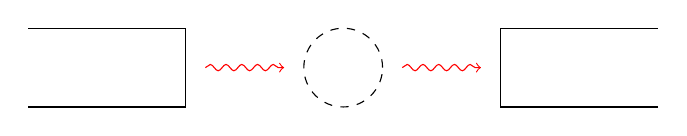
\begin{tikzpicture}

\draw (0,0) -- (2,0) -- (2,1) -- (0,1);
\draw[red, ->,decorate,decoration={snake,amplitude=.4mm,segment length=2mm}] (2.25,0.5) -- (3.25,0.5);
\draw[dashed] (4,0.5) circle (0.5);
\draw[red, ->,decorate,decoration={snake,amplitude=.4mm,segment length=2mm}] (4.75,0.5) -- (5.75,0.5);
\draw (8,0) -- (6,0) -- (6,1) -- (8,1);

\end{tikzpicture}
~\\
~\\
~\\
Controlled tunneling of electrons through the dot:\\
- Input\\
- Coulomb blockade\\
- Spin (Pauli) blockade\\
- Readout

\end{frame}

\begin{frame}[t]\frametitle{Contents}

Quantum dot \\
  - Coulomb blockade \\
  ~\\
Mean-field method for these and similar actions\\
  - Decoupling through Hubbard-Stratonovich transformation \\
  - Integrate over fermionic degrees of freedom \\
  - Stationary phase approximation of auxiliary field \\
  - Effective action

\end{frame}

\begin{frame}[t]\frametitle{Coulomb blockade}
Action
\begin{align*}
S[\bar{\Psi}_{\alpha}, \Psi_{\alpha}] = \sum_{\alpha} \bar{\psi}_{\alpha} (\partial_{\tau} + \epsilon_{\alpha} - \mu) \psi_{\alpha}
 + E_C (\sum_{\alpha} \bar{\Psi}_{\alpha} \Psi_{\alpha} - N_0)^2
\end{align*}

Hubbard-Stratonovich transformation:
\begin{align*}
\psi^4 \to \psi^2 V + V^2 + V
\end{align*}
In this case
\begin{align*}
e^{-E_C (\sum_{\alpha} \bar{\Psi}_{\alpha} \Psi_{\alpha} - N_0)^2 }
  = \int DV ~ e^{-\frac{V^2}{4 E_C} + i N_0 V - i \sum_{\alpha} \bar{\Psi}_{\alpha} V \Psi_{\alpha}}
\end{align*}
\end{frame}

\begin{frame}[t]\frametitle{Coulomb blockade}
This leads to
\begin{align*}
&G_{\alpha} = \frac{1}{Z} \int D(\bar{\psi}, \psi) e^{-\Cline[purple]{S_{free}[\bar{\psi}, \psi]}-\Cline[green]{S_{int}[\bar{\psi}, \psi]}}\bar{\psi}_{\alpha} \psi_{\alpha}\\
  &= \frac{1}{Z} \int D(\bar{\psi}, \psi) e^{-\Cline[purple]{\sum_{\alpha} \bar{\psi}_{\alpha} (\partial_{\tau} + \epsilon_{\alpha} - \mu) \psi_{\alpha}}
 - \Cline[green]{E_C (\sum_{\alpha} \bar{\Psi}_{\alpha} \Psi_{\alpha} - N_0)^2}} \bar{\psi}_{\alpha} \psi_{\alpha} \\
 &= \frac{1}{Z} \int DV ~ e^{-S[V]} \int D(\bar{\psi}, \psi) e^{-\Cline[purple]{\sum_{\alpha} \bar{\psi}_{\alpha} (\partial_{\tau} + \epsilon_{\alpha} - \mu \textcolor{green}{+ i V}) \psi_{\alpha}
  }} \bar{\psi}_{\alpha} \psi_{\alpha}\\
  &= \frac{1}{Z} \int DV ~ e^{-S[V]} \int D(\bar{\psi}, \psi) e^{-S^V[\bar{\psi}, \psi]}\bar{\psi}_{\alpha} \psi_{\alpha}
\end{align*}
\begin{align*}
  S^V[\bar{\psi}, \psi] = S_{free}[\bar{\psi}, \psi]\rvert_{\mu \to \mu - i V}
\end{align*}

\end{frame}

\begin{frame}[t]\frametitle{Coulomb blockade}

  Using a gauge transformation of the form
  \begin{align*}
    \psi(\tau) \to \psi(\tau) e^{-i \int^{\tau} d\tau' (V(\tau') - V_0)}
  \end{align*}
  The action $S^V$ can be reduced
  \begin{align*}
    S^V[\bar{\psi}, \psi] \to S^{V_0}[\bar{\psi}, \psi]
  \end{align*}
  At the cost of an extra gauge factor
  \begin{align*}
    \frac{1}{Z} \int DV ~ e^{-S[V]} \int D(\bar{\psi}, \psi) e^{-S^{V_0}[\bar{\psi}, \psi]} ~ \textcolor{green}{e^{-i \int^{\tau} d\tau' (V(\tau') - V_0)}} ~ \bar{\psi}_{\alpha} \psi_{\alpha}
  \end{align*}

\end{frame}

\begin{frame}[t]\frametitle{Coulomb blockade}
  The integral over the auxiliary field can be split
  \begin{align*}
    \int DV = \prod_{n=0} \int dV_n = \int dV_0 \prod_{n=1} \int dV_n
  \end{align*}

  The integration over de $V_n$ components gives a Matsubara summation
  \begin{align*}
    -2 E_C T \sum_{n \not= 0} \frac{1}{\omega_n^2} (1 - e^{-i \omega_n \tau})
    = - E_C (|\tau| - T \cdot \tau^2)
  \end{align*}
  \emph{Note:} this is not a trivial calculation, but the answer is obtained by using
  \begin{align*}
    \sum_{k=1}^{\infty} \frac{cos(k x)}{k^2} \approx \frac{\pi^2}{6} - \frac{\pi |x|}{2} + \frac{x^2}{4}
  \end{align*}
\end{frame}

\begin{frame}[t]\frametitle{Coulomb blockade}
  In our action, we can write
  \begin{align*}
    G(\tau) &= \frac{1}{Z} \int DV ~ e^{-S[V]} \int D(\bar{\psi}, \psi) ~ e^{-i \int^{\tau} d\tau' (V(\tau') - V_0)} ~ e^{-S^{V_0}[\bar{\psi}, \psi]} ~ \bar{\psi}_{\alpha} \psi_{\alpha}\\
    &= \frac{1}{Z} \int DV ~ e^{-S[V]}  ~ e^{-i \int^{\tau} d\tau' (V(\tau') - V_0)} Z^{V_0} G_{\alpha}^{V_0}\\
    &= \frac{F(\tau)}{Z} \int dV_0 ~ e^{-S[V_0]} Z^{V_0} G_{\alpha}^{V_0}
  \end{align*}
  Where
  \begin{align*}
    F(\tau) \equiv e^{- E_C (|\tau| - T \cdot \tau^2)}
  \end{align*}
\end{frame}

\begin{frame}[t]\frametitle{Coulomb blockade}
  In
  \begin{align*}
    G(\tau) &= \frac{F(\tau)}{Z} \int dV_0 ~ e^{-S[V_0]} Z^{V_0} G_{\alpha}^{V_0}
  \end{align*}
  We can define a free energy $\mathcal{F}(\mu)$ as
  \begin{align*}
    Z^{V_0} = e^{-\beta ~ \mathcal{F}^{V_0}(\mu)} = e^{-\beta ~ \mathcal{F}(\mu - i V_0)}
  \end{align*}
  So we have, writing out the $S[V_0]$:
  \begin{align*}
    G(\tau) &= \frac{F(\tau)}{Z} \int dV_0 ~ e^{-\frac{\beta}{4 E_C} V_0^2 + i \beta N_0 V_0 - \beta ~ \mathcal{F}(\mu - i V_0)} G_{\alpha}^{V_0}
  \end{align*}
  which can be approximated using the stationary phase method
\end{frame}

\begin{frame}[t]\frametitle{Stationary phase approximation}
  When given an integral of the form
  \begin{align*}
    I = \lim_{\lambda \to \infty} \int_{-\infty}^{-\infty} e^{-\lambda f(x)}
  \end{align*}
  The relevant contributions occur around minimum $x_0$ of $f$:
  \begin{align*}
    \left.\frac{\partial f}{\partial x} \right\rvert_{x = x_0} = 0
  \end{align*}
  Which is known as the \emph{saddle point equation}
\end{frame}

\begin{frame}[t]\frametitle{Stationary phase approximation}
  In the case of our action, we have the exponent
  \begin{align*}
    -\frac{\beta}{4 E_C} V_0^2 + i \beta N_0 V_0 - \beta ~ \mathcal{F}(\mu - i V_0)
  \end{align*}
  Which has a minimum (after some calculation)
  \begin{align*}
    0 = \frac{1}{2 E_C} V_0 - i N_0 + i \left<\hat{N}\right>_{\mu - i V_0}
  \end{align*}
  where we used that
  \begin{align*}
    \frac{\partial}{\partial V_0} \mathcal{F}(\mu - i V_0) = - i \frac{\partial}{\partial \mu} \mathcal{F}(\mu - i V_0) = - i \left<\hat{N}\right>_{\mu - i V_0}
  \end{align*}

  where $\hat{N}$ is the number operator
  \begin{align*}
    \hat{N} \equiv \sum_{\alpha} a_{\alpha}^{\dagger} a_{\alpha}
  \end{align*}

\end{frame}

\begin{frame}[t]\frametitle{Density of states}
  Filling in the solutions, we can calculate the tunneling density of states by
  \begin{align*}
    \nu(\epsilon) = - \frac{1}{\pi} Im~tr~G
  \end{align*}
  After some calculations, we obtain
  \begin{align*}
    \nu(\epsilon) = \nu_0(\epsilon - E_C ~ sgn(\epsilon)) ~ \Theta(|\epsilon| - E_C)
  \end{align*}
  Where $\nu_0$ is the density of states (shifted by the energy cost) of the non-interacting systems and $\Theta$ a step function.\\
  ~\\
  This means that there is an energy gap of size $2 E_C$ around the Fermi energy


\end{frame}

\begin{frame}[t]\frametitle{Conclusions}
  The Coulomb blockade prevents electrons of certain energies to tunnel into the dot. \\
  ~\\
  If it has energy $\epsilon > E_C$ it is allowed to tunnel

  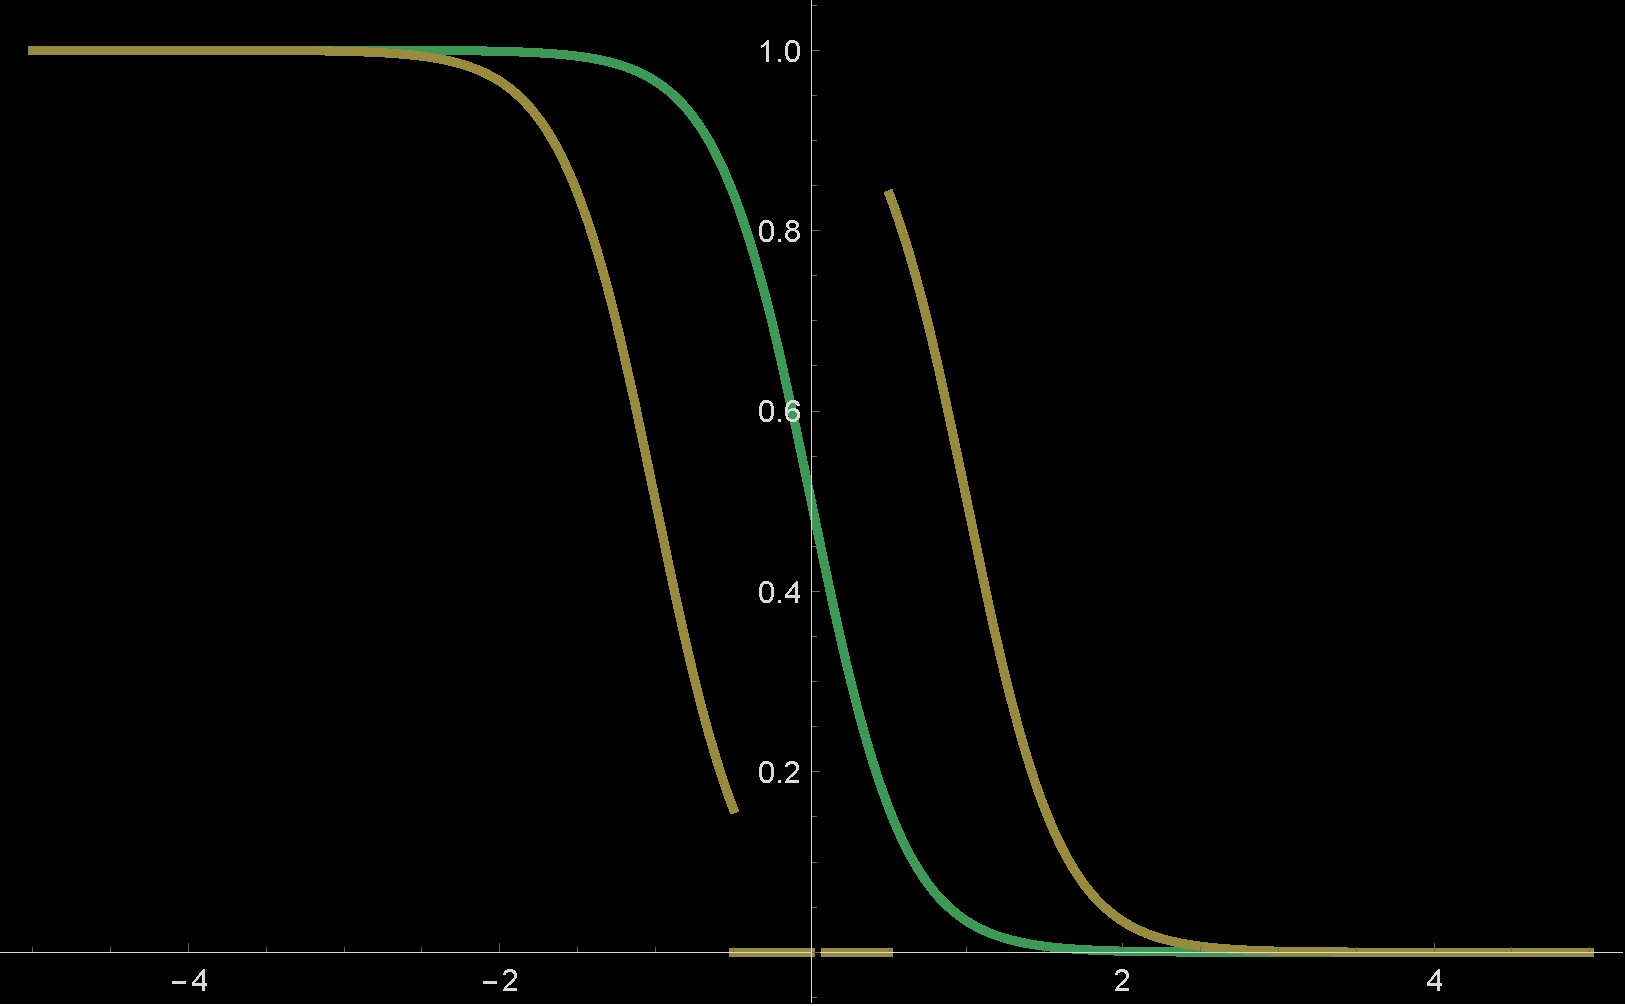
\includegraphics[scale=0.35]{plt_fd}
\end{frame}

\end{document}
